\documentclass{article}

% ready for submission
\usepackage[final]{neurips_2023}
\usepackage{amsmath}
\usepackage{graphicx}
\usepackage{float}
\usepackage{subfig}         % display sub-figure
\usepackage[utf8]{inputenc} % allow utf-8 input
\usepackage[T1]{fontenc}    % use 8-bit T1 fonts
\usepackage{hyperref}       % hyperlinks
\usepackage{url}            % simple URL typesetting
\usepackage{booktabs}       % professional-quality tables
\usepackage{amsfonts}       % blackboard math symbols
\usepackage{nicefrac}       % compact symbols for 1/2, etc.
\usepackage{microtype}      % microtypography
\usepackage{xcolor}         % colors

\title{Dynamic Daytime Simulation with Accumulated Snow Effect}

\author{%
  Steven Webb\\\\
  u7544998 
   \And
  Leosha Trushin\\\\
  u7302755\\
  \AND  The Australian National University 
}

\begin{document}

\maketitle

\begin{abstract}
TODO:
\end{abstract}

% 1. Introduction
\section{Introduction}
Snow rendering and daytime simulation are two important applications in the Computer Graphics fields. Both of them can be used in 
other applications like video games, movies and virtual reality. Snow is one of the most valuable natural resources and it is also
important to render it in the Computer Graphics applications. There are two major kinds of snow rendering, which are falling snow 
which is based on particles floating in the air [1], and accumulated snow covering objects. The snow rendering type in his paper 
is the accumulated snow.

Daytime simulation is also an important field in Computer Graphics. For instance, many 3D video games require a robust daytime 
simulation system to calculate the sunlight/moonlight position, intensity and color. This can also change the color of the sky and all  
relevant scenes, providing players with an immersive gaming experience. The daytime simulation also has a strong connection with snow 
rendering as it determines the snow color in the eye view. This paper will implement both accumulated snow rendering and a dynamic
daylight system, as well as the connections between them.
% 1. Introduction

\section{Background}

\section{Motivations}

\section {Methods}

% Method part 1: Snow Rendering
\subsection {Snow Rendering}

% Snow method 1: Color
\subsubsection {Snow Color Function}
The snow color is based on the Phong reflection model with the following modifications.

%where:
\begin{itemize}
  % TODO: REF
  \item The diffuse reflection coefficient \( k_d \) becomes a fixed value, which is the snow color. To make a more glittering effect, the 
  blue component of it can be slightly higher. In this paper, \( k_d = (0.9375, 0.9375, 1)\)
  \item A distortion is added to the surface normal \( N \). In the modified model, \( N = N_{o} + \alpha * n\), where \( \alpha \) is 
  the distortion coefficient and \( n \) is a random vector. In this paper, \( \alpha = 0.1\).
  \item The specular exponent \( \beta \) is a small value to make sure snow is not very shiny. In this paper, \( \beta = 25\).
\end{itemize}

% Snow method 2: Accumulation Prediction Coefficient
\subsubsection {Snow Accumulation Prediction Coefficient}
Assume there is no wind in the scene and all snow falls vertically. The snow accumulation prediction coefficient \( f_{s} \) on a 
point can be calculated by the multiplication of an exposure value \( f_{e} \), an inclination value \( f_{inc} \), and a user-defined 
value \( f_{u} \).
\[
  f_{s} = f_{e} \cdot f_{inc} \cdot f_{u}
\]

% TODO: REF
The exposure value \( f_{e} \in [0, 1] \) indicates occlusions that prevent snow from falling on the surface. \( f_{e}=0 \) means that 
the point is fully occluded by an above object, and there are no snowing effects on this point. \( f_{e}=1 \) means that the point is 
fully exposed to the falling snow. This value is based on a shadow map by setting a virtual directional light right above the object. 
The light direction is to the ground, so the points in the virtual shadow are also occluded by an object. Besides, to make the 
transition process smoother, soft shadowing techniques can be used. 

The inclination value \( f_{inc} \in [0, 1] \) depends on the angle between the surface normal and the horizon. \( f_{inc}=1 \) means 
that the point is on a flat surface that is parallel to the horizon. \( f_{inc}=0 \) indicates that the point is on a surface which is 
perpendicular to the horizon. This value can be calculated by:
\[
  f_{inc}=
  \left\{
    \begin{array}{ll}
      N \cdot U + n & N \cdot U > 0 \\
      0 & N \cdot U \leq 0 \\
    \end{array} 
  \right. 
\]

where:
\begin{itemize}
  \item \( N \) is the surface normal of the target point (normalized).
  \item \( U \) is the surface normal of the horizon (normalized). It is a constant vector \((0, 0, 1)\)
  \item \( N \cdot U \) is the cosine of the angle between the above two surface normals, ranging from -1 to 1. If the angle is less 
  than 90$^{\circ}$, \( N \cdot U > 0\).
  \item \( n \) is a small random number to make snow have a more natural look. In this paper, \(n = rand(0, 0.4)\).
\end{itemize}

Figure 1 is the visualization of the occlusion and inclination map with legends. 

\begin{figure}[h]
  \centering
  \subfloat[Occlusion Map]{
    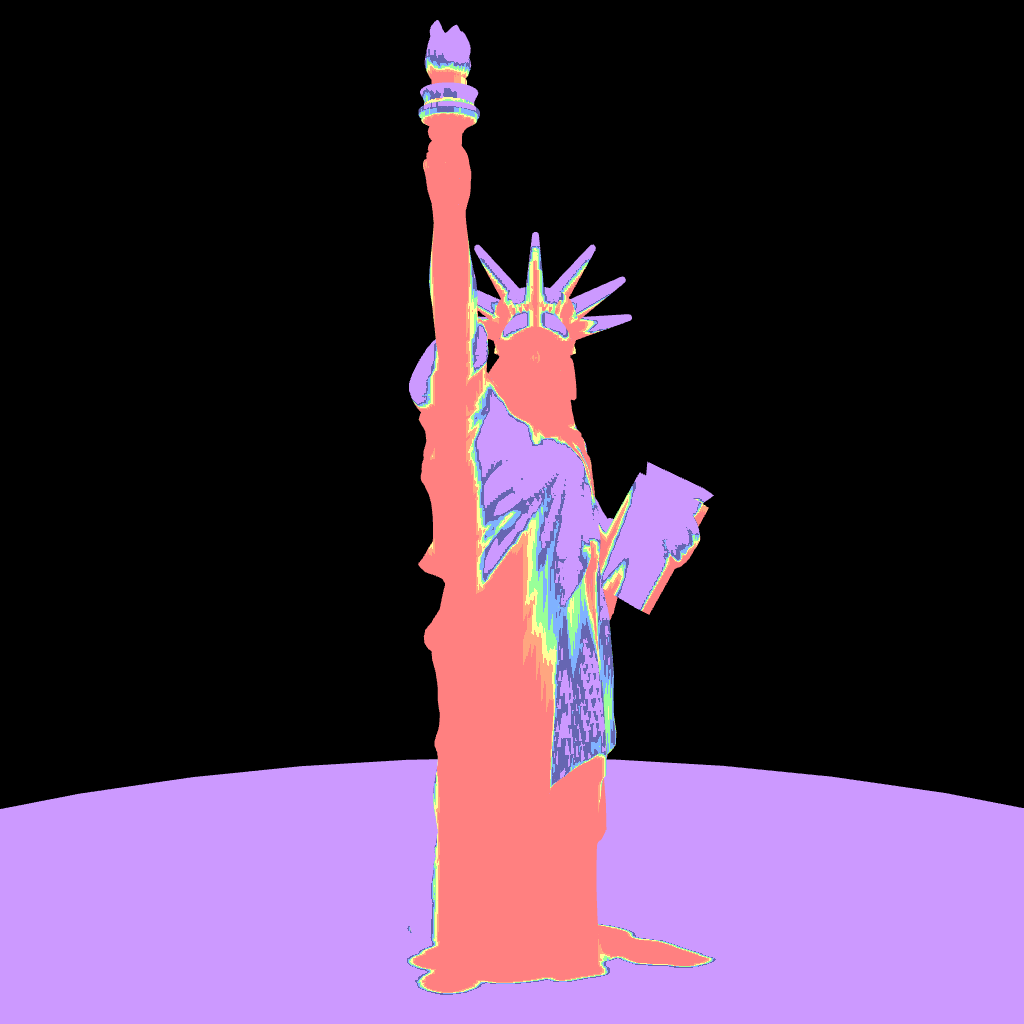
\includegraphics[width=0.33\textwidth]{images/MapOcclusion.png}
    \label{fig:MapOcclusion}
  }
  \subfloat[Inclination Map]{
    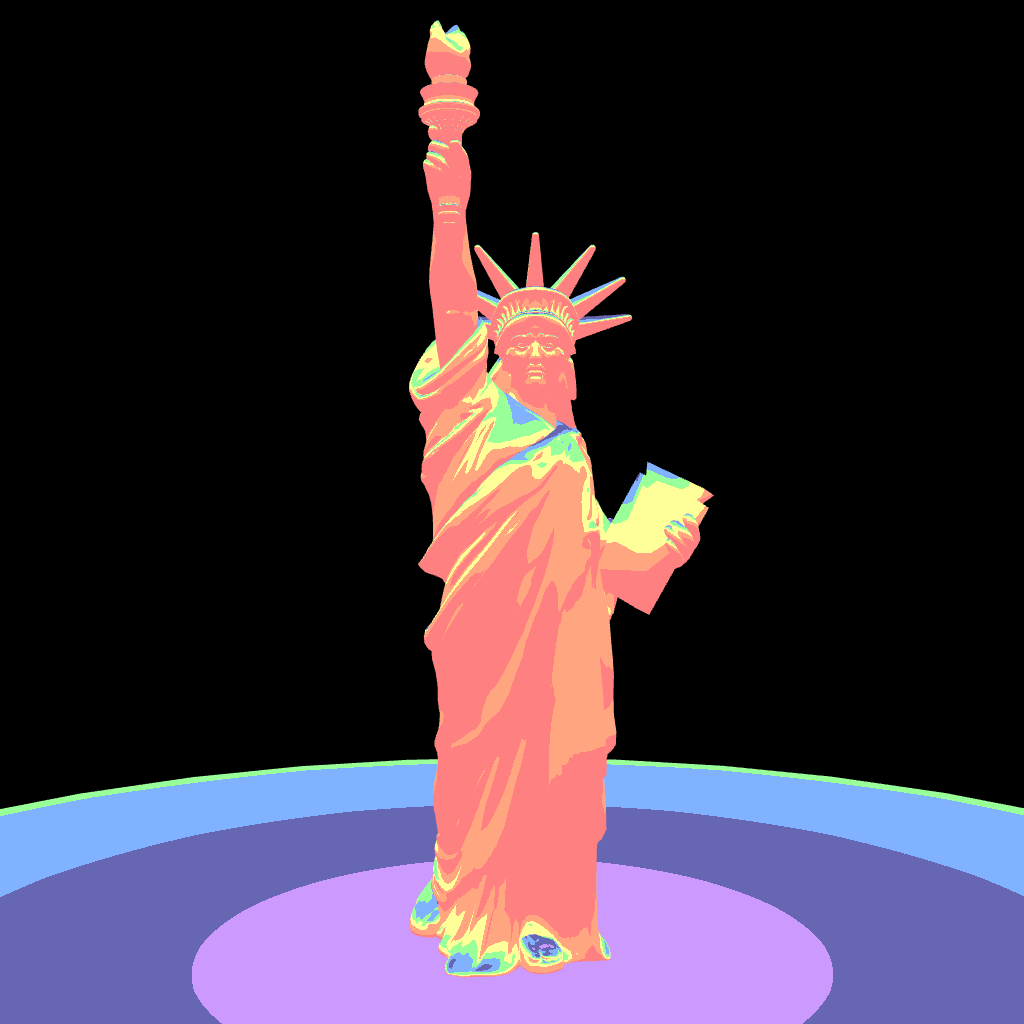
\includegraphics[width=0.33\textwidth]{images/MapInclination.png}
    \label{fig:MapInclination}
  }
  \subfloat[Legend of Maps]{
    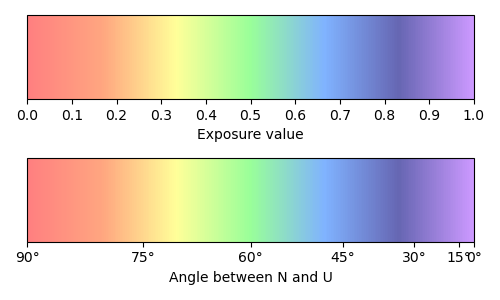
\includegraphics[width=0.33\textwidth]{images/MapLegend.png}
    \label{fig:MapLegend}
  }
  \caption{Occlusion and Inclination Map}
  \label{fig:Maps}
\end{figure}



The user-defined function \( f_{u} \in [0, 1]\) is used to further customize and manipulate the snow amount. For example, 
\( f_{u}=0 \) means manually disabling the snow effect. This function is crucial in the daytime simulation.

% Snow method 3: Full Snow Equation
\subsubsection {Full Snow Equation}
The final color \( C \) is a blending of the snow color and the surface color (without snow) on that point, by using the snow accumulation 
prediction coefficient in the last sub-section. This is also called the "Full Snow Equation".
\[
  C = f_{s} * C_{s} + (1-f_{s}) * C_{o}
\]

where:
\begin{itemize}
  \item \( f_{s} \) is the snow accumulation prediction coefficient.
  \item \( C_{s} \) is the snow color.
  \item \( C_{o} \) is the surface color without snow.
\end{itemize}

% Method part 2: Environment Simulation
\subsection {Environment Simulation}

% Environment 1: Temperature
\subsubsection {Temperature}
The temperature curve in this paper is based on the real temperature of an in-land city around the latitude of 35$^{\circ}$ N or 35
$^{\circ}$ S in winter solstice day. This location has a large temperature difference. The highest temperature is about 
\(10^\circ\mathrm{C}\), which happens at around 1-2 P.M. The lowest temperature is about \(-10^\circ\mathrm{C}\), which can be reached 
at around 5-7 A.M. The hourly temperature data is obtained on a weather forecast website, and the Cubic Spline method is used to 
interpolate the intermediate values, making the curve smoother.
% Environment 1: Temperature

% Environment 2: Snow Factor
\subsubsection {Snow Factor}
The snow factor is the user-defined function \( f_{u} \) in Section 4.1, making a potentially negative effect on the original snow. To 
simplify the simulation, this is based solely on the environmental temperature. If the temperature \( t \leq 0^\circ\mathrm{C}\), the 
snow factor is always 1. If \( t \geq 5^\circ\mathrm{C}\), the snow factor is always 0. Otherwise, the snow factor decreases linearly 
from 1 to 0 as temperature increases.
\[
  f_{u}=
  \left\{
    \begin{array}{ll}
      0 & t\leq 0 \\
      1 - \frac{t}{5} &  0 < t < 5 \\
      1 & t\geq 5 \\
    \end{array} 
  \right. 
\]
% Environment 2: Snow Factor

% Environment 3: Sunlight Intensity and Direction
\subsubsection {Sunlight Intensity and Direction}
In this paper, only the sunlight and sky (ambient) light are considered. The intensity of the skylight is a small constant value 
while that of the sunlight varies by time, ranging from 0 to 1. Assume the light intensity of the sun is 0 at night. It starts 
increasing rapidly (typically 30 minutes) before sunrise and reaches the maximum value in a short time (typically 1-3 hours). It 
remains stable until several hours before the sunset. The value decreases quickly in the sunset period and finally returns to 0. Here 
is the mathematical formula of the light intensity \( I \in (0, 1]\), which is based on a bell curve.
\[
  I = e^{-\frac{\left(\frac{\pi}{2} - \theta\right)^{\frac{m}{60} + 1}}{b}}
\]

where:
\begin{itemize}
  \item \( \theta \) is the solar elevation angle in radians, which is based on the current time, season (Earth declination) and 
  position (latitude).
  \item \( m \in [0, 1440)\) \( m \in \mathbb{Z} \) is the total daylight time (in minutes) on that day. For example, if the sunrise 
  time is 6 AM and the sunset time is 6 PM, \( m=720 \) (12 hours).
  \item \( b \) is a bias factor adjusting the exponent decay rate, making the light intensity transition more realistic.
\end{itemize}

The bias \( b \) depends on multiple factors, including the location and time zone. A simple approach to estimate it is to solve an 
equation in terms of \( m \) when \( I \) and \( \theta\) is given. For example, if \( I=0.1 \) on sunrise or sunset (i.e., 
\( \theta=0\)), the formula of the bias is:
\[
  b = \frac{\left(\frac{\pi}{2}\right)^{\frac{m}{60} + 1}}{\log(10)}
\]

By giving the sun elevation angle \( \theta \) and azimuth angle \( \phi \), the sunlight direction can be calculated by:
\[
  (-sin(\phi)cos(\theta), -cos(\phi)cos(\theta), sin(\theta))
\]
% Environment 3: Sunlight Intensity and Direction

% Environment 4: Sunlight and Sky Color
\subsubsection {Sunlight and Sky Color}
Sunlight and sky colors depend on the current time. Typically on a sunny day, the sunlight is yellow to white for most of the day and 
it becomes orange during sunrise or sunset. The sky is light blue in the day, orange during sunrise or sunset and dark purple at night. 
To simulate those colors, interpolation is also needed to make the transition process smoother. 
\[
  C_{b}=
  \left\{
    \begin{array}{ll}
      \text{night} & \theta \leq 10 \\
      \text{interpolate(night, twilight)} &  -10 \leq t < 5 \\
      \text{interpolate(twilight, day)} &  5 \leq t < 20 \\
      \text{day} & t \geq 20 \\
    \end{array} 
  \right. 
\]
% Environment 4: Sunlight and Sky Color

\section{Results}

% Result 1: Pure Snow Effect
\subsection {Pure Snow Effect}
Figure 2 is the rendering effect with full snow (a), half snow (b), and no snow (c) respectively. The dynamic daylight simulation is 
disabled and the light source is always right above the object with the maximum intensity and white color. Those three sub-figures 
illustrate the effect on both declination (the head and book part of the statue) and occlusion (the feet area of it), as well as the 
color blending mentioned above.

\begin{figure}[h]
  \centering
  \subfloat[Snow Amount = 1.0]{
    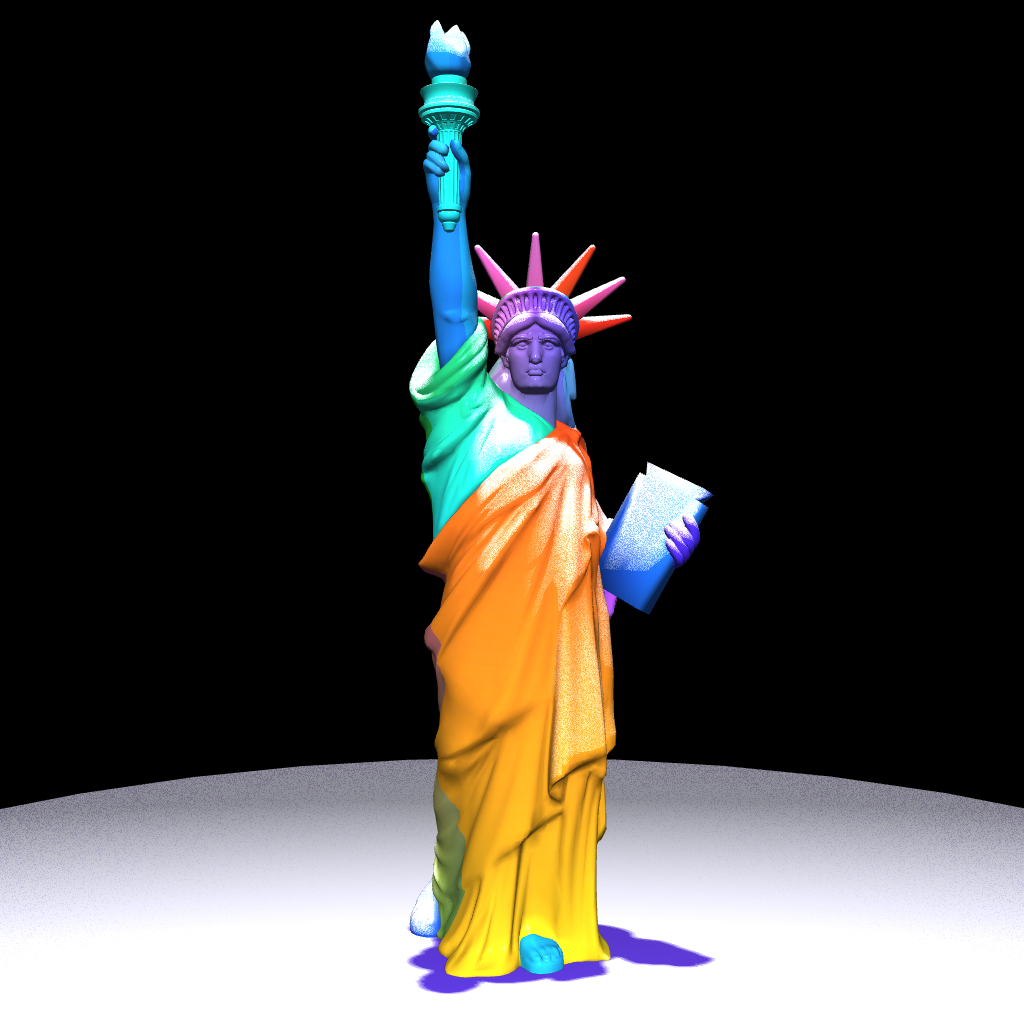
\includegraphics[width=0.33\textwidth]{images/T9999M10P.png}
    \label{fig:T9999M10P}
  }
  \subfloat[Snow Amount = 0.5]{
    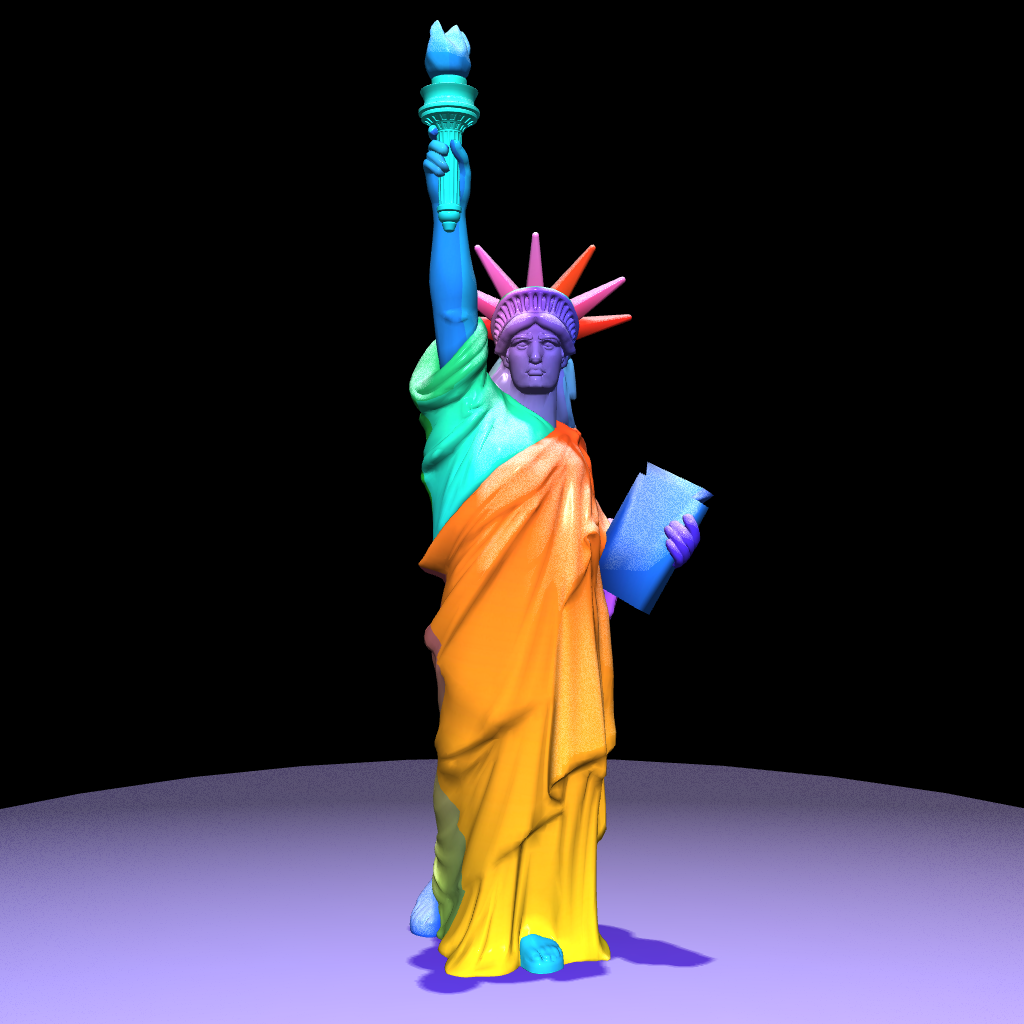
\includegraphics[width=0.33\textwidth]{images/T9999M05P.png}
    \label{fig:T9999M05P}
  }
  \subfloat[Snow Amount = 0.0]{
    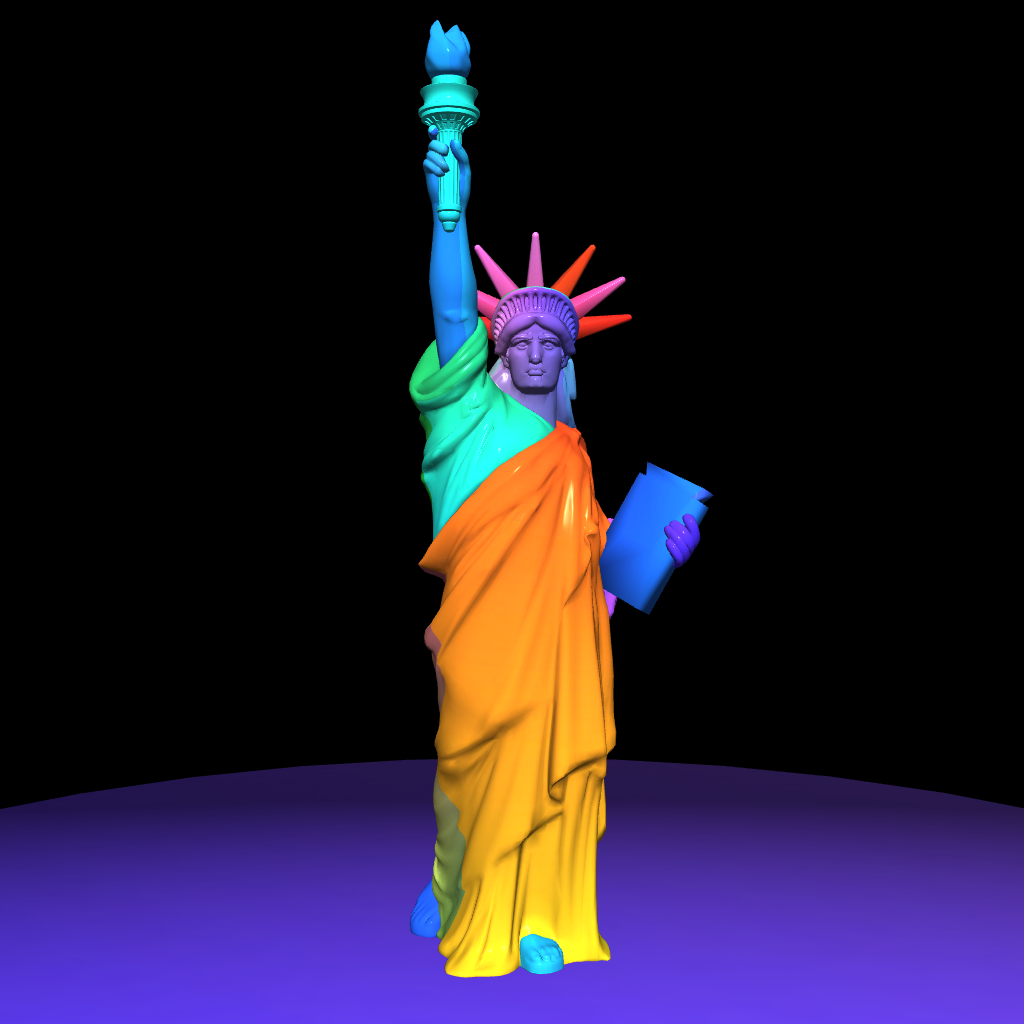
\includegraphics[width=0.33\textwidth]{images/T9999M00P.png}
    \label{fig:T9999M00P}
  }
  \caption{Object covered by different amounts of snow}
  \label{fig:PureSnow}
\end{figure}
% Result 1: Pure Snow Effect

% Result 2: Snow Effect with Dynamic Daylight Simulation (Medium Latitude)
\subsection {Snow Effect with Dynamic Daylight Simulation (Medium Latitude)}

Figure 3 is the plot of the data at different times with a medium latitude location on the winter solstice (35 $^{\circ}$S on June 
\(22^{nd}\)). The sunrise time is about 7:00 AM and the sunset time is about 5:00 PM, so there are 10 hours of daylight time.

\begin{figure}[h]
  \centering
  \begin{minipage}{1.00\textwidth}
      \centering
      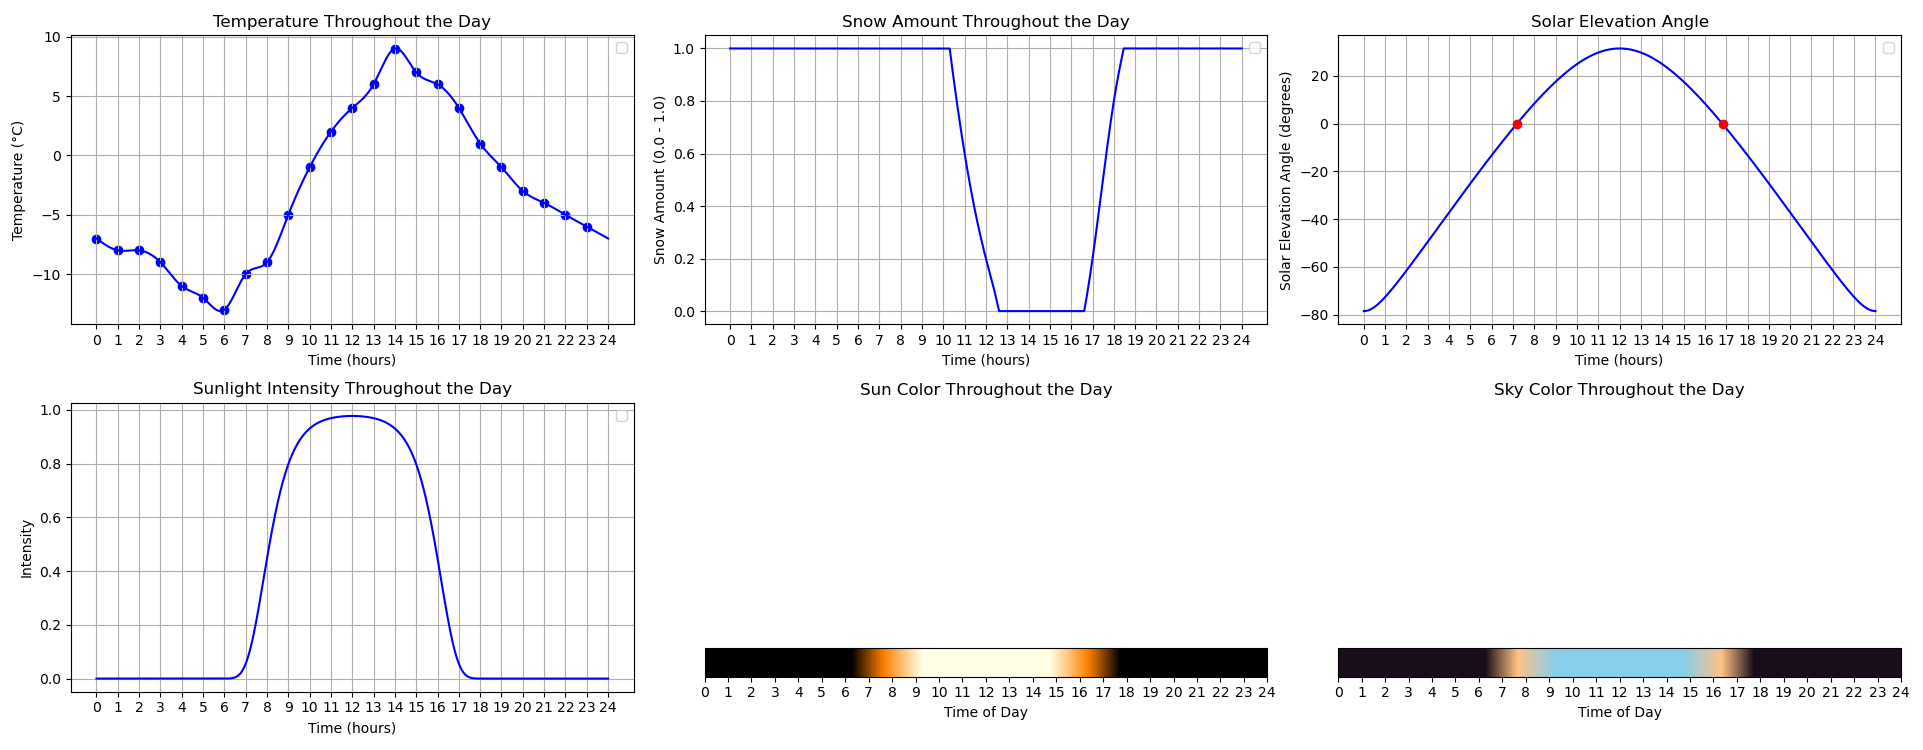
\includegraphics[width=\textwidth]{images/Plot35N.png}
      \caption{Relevant data in 35 $^{\circ}$S on June \(22^{nd}\)}
      \label{fig:Plot35N}
  \end{minipage}
\end{figure}

Figure 4 shows the rendering effect at different times. Throughout the night (e.g., midnight (a) or 7:00 PM (f)), the object is fully 
covered by white snow and only ambient colors can be seen due to low temperature and sunlight intensity. In the morning (e.g., 8:00 
AM (b)), the sunlight intensity increases with an orange color, changing the sky and snow color. The snow coverage is still 100 \% due
to the low temperature. 

Around noon (e.g., 11:00 AM (c)), the sky becomes light blue and the snow (back to white color) starts melting at this time. Part of 
the covered object can be seen now. In the afternoon (e.g., 2:00 PM (d)), there is no snow on the scene thanks to the warm temperature. 
During the sunset period, (e.g., 5:00 PM (e)), the sunlight intensity drops back and the sunlight color/sky color becomes orange again. 
The snow effect is back due to the dropping temperature.

\begin{figure}[h]
  \centering
  \subfloat[Time = 12:00 AM]{
    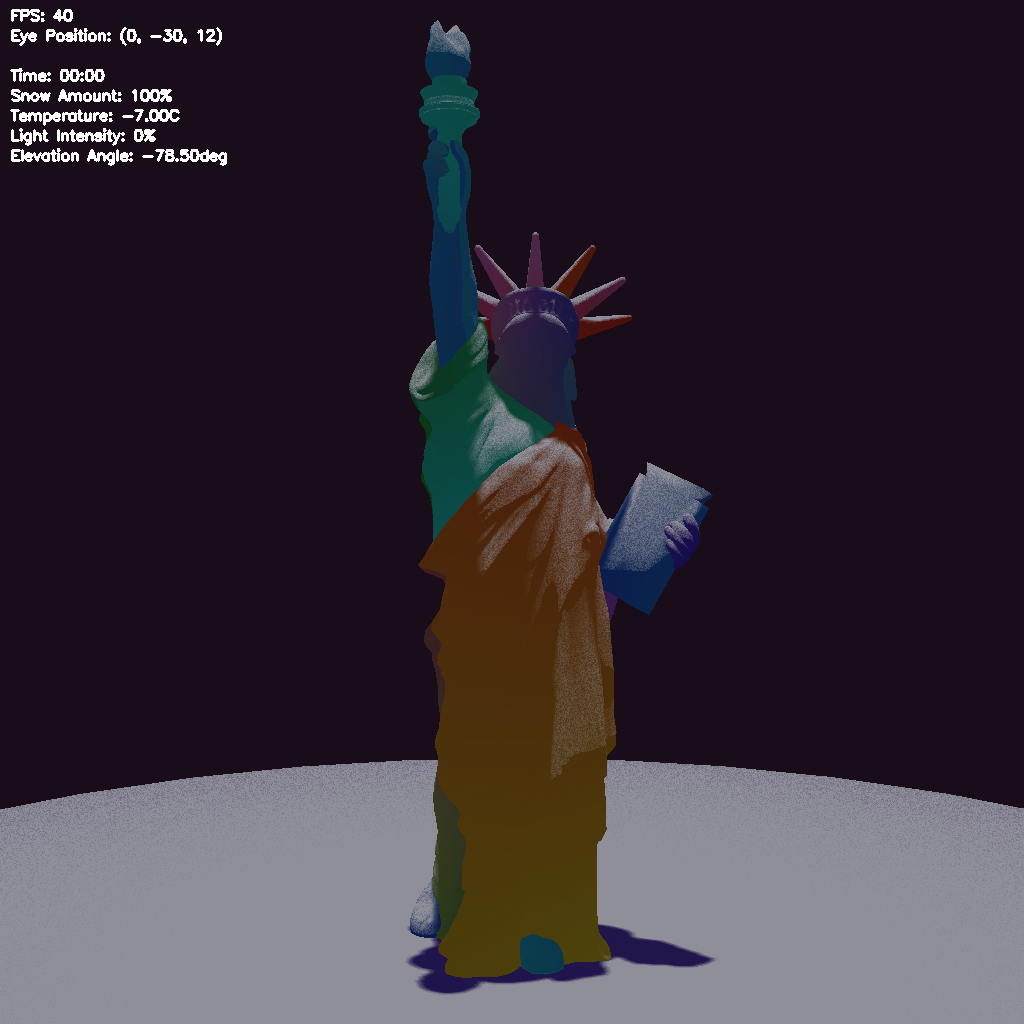
\includegraphics[width=0.33\textwidth]{images/T0000L35S.png}
    \label{fig:T0000L35S}
  }
  \subfloat[Time = 08:00 AM]{
    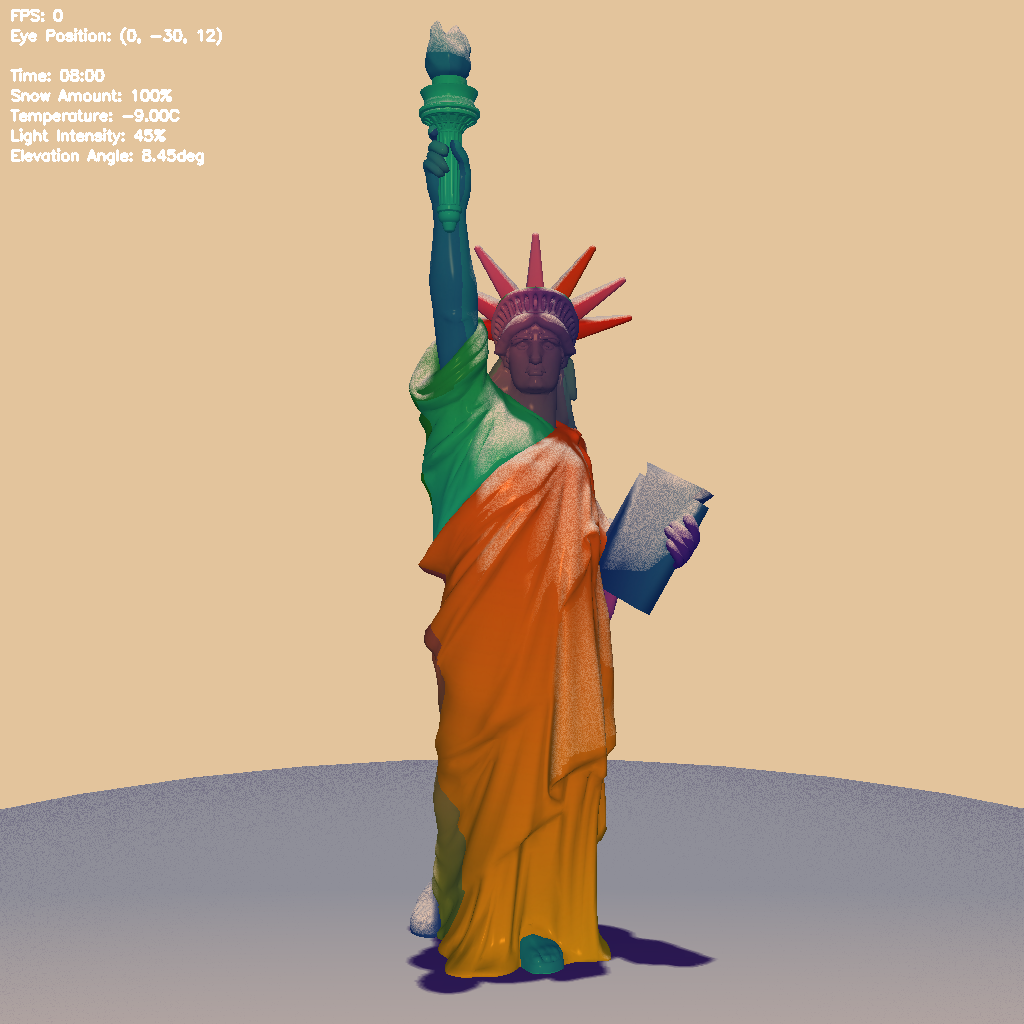
\includegraphics[width=0.33\textwidth]{images/T0800L35S.png}
    \label{fig:T0800L35S}
  }
  \subfloat[Time = 11:00 AM]{
    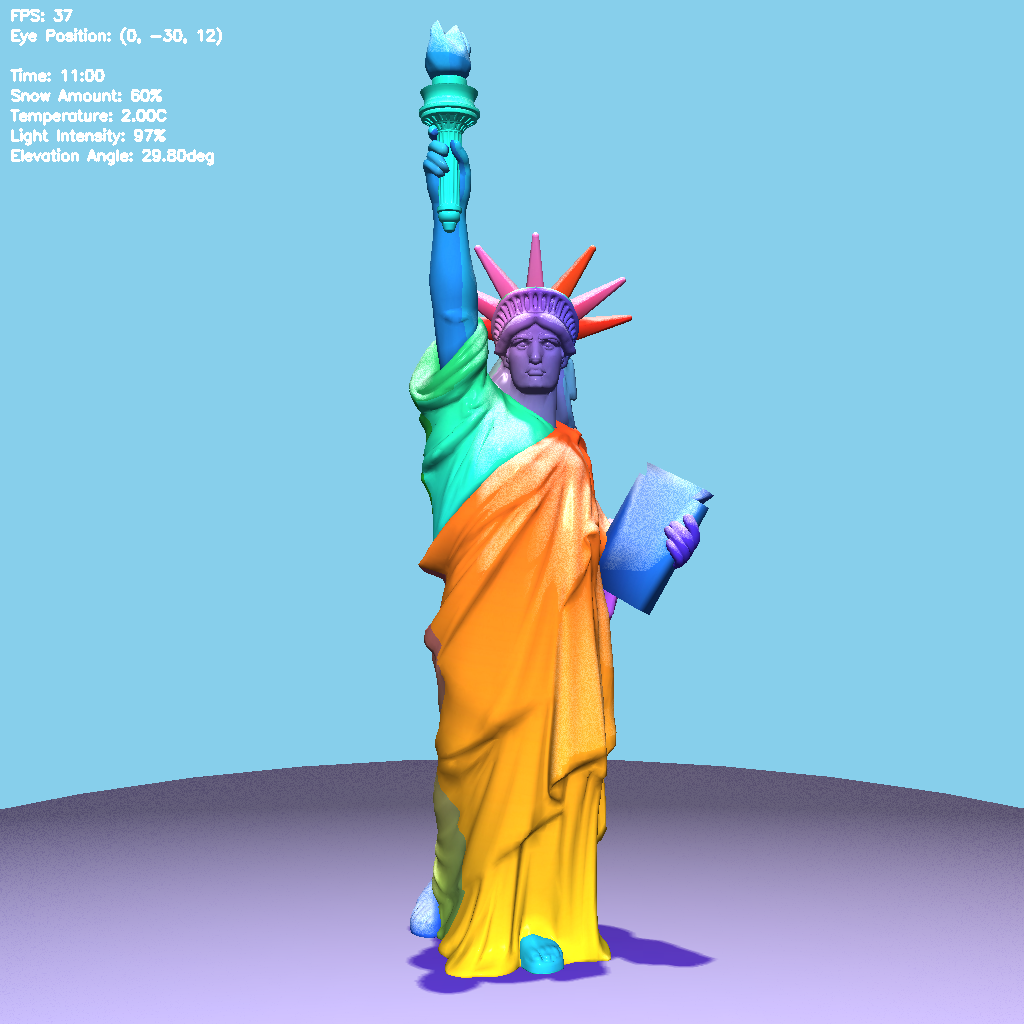
\includegraphics[width=0.33\textwidth]{images/T1100L35S.png}
    \label{fig:T1100L35S}
  }

  \subfloat[Time = 02:00 PM]{
    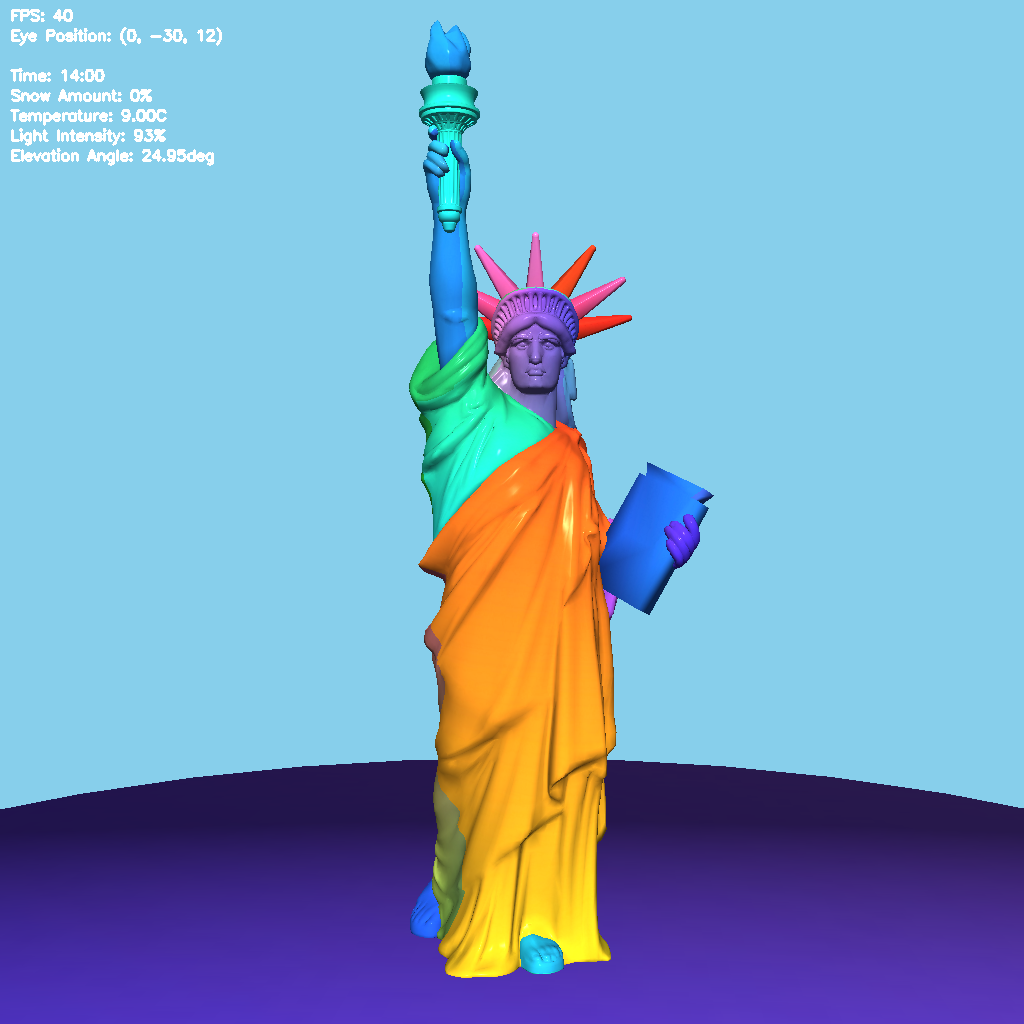
\includegraphics[width=0.33\textwidth]{images/T1400L35S.png}
    \label{fig:T1400L35S}
  }
  \subfloat[Time = 05:00 PM]{
    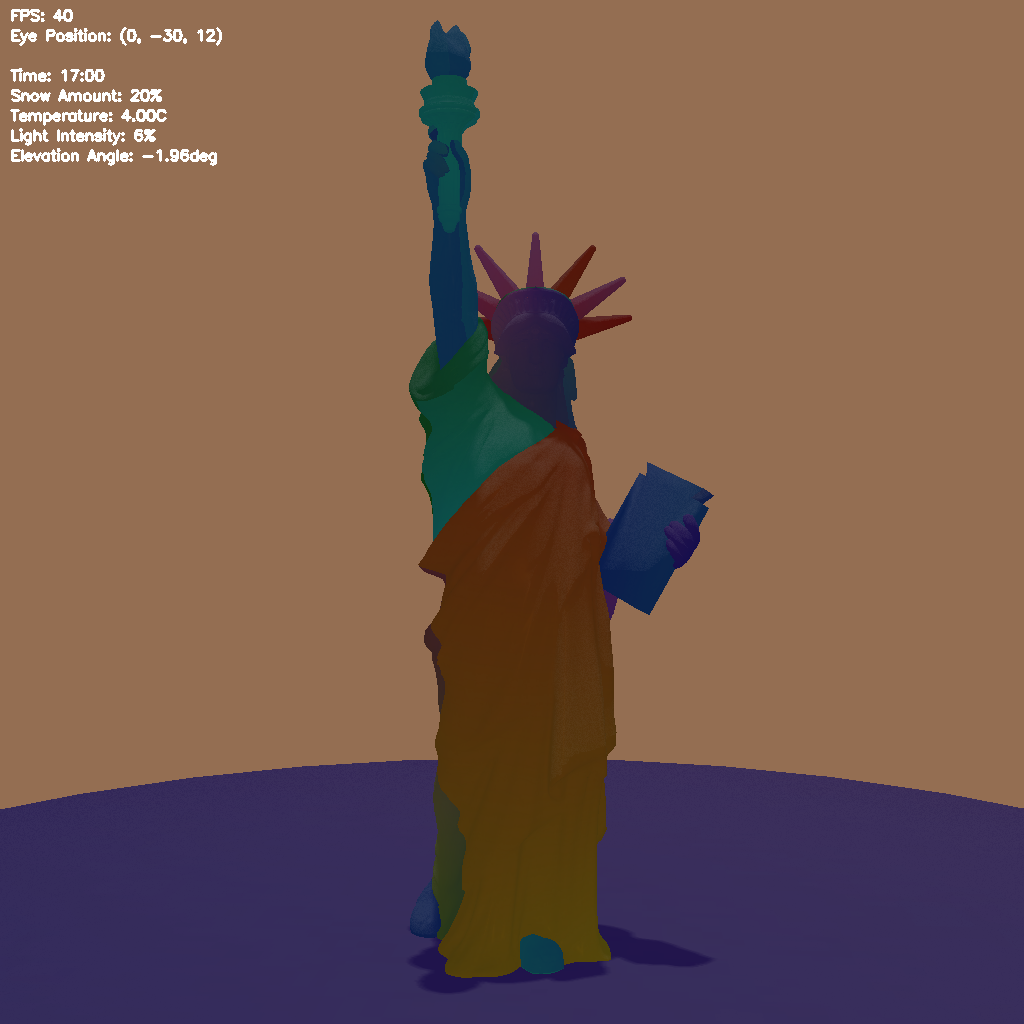
\includegraphics[width=0.33\textwidth]{images/T1700L35S.png}
    \label{fig:T1700L35S}
  }
  \subfloat[Time = 07:00 PM]{
    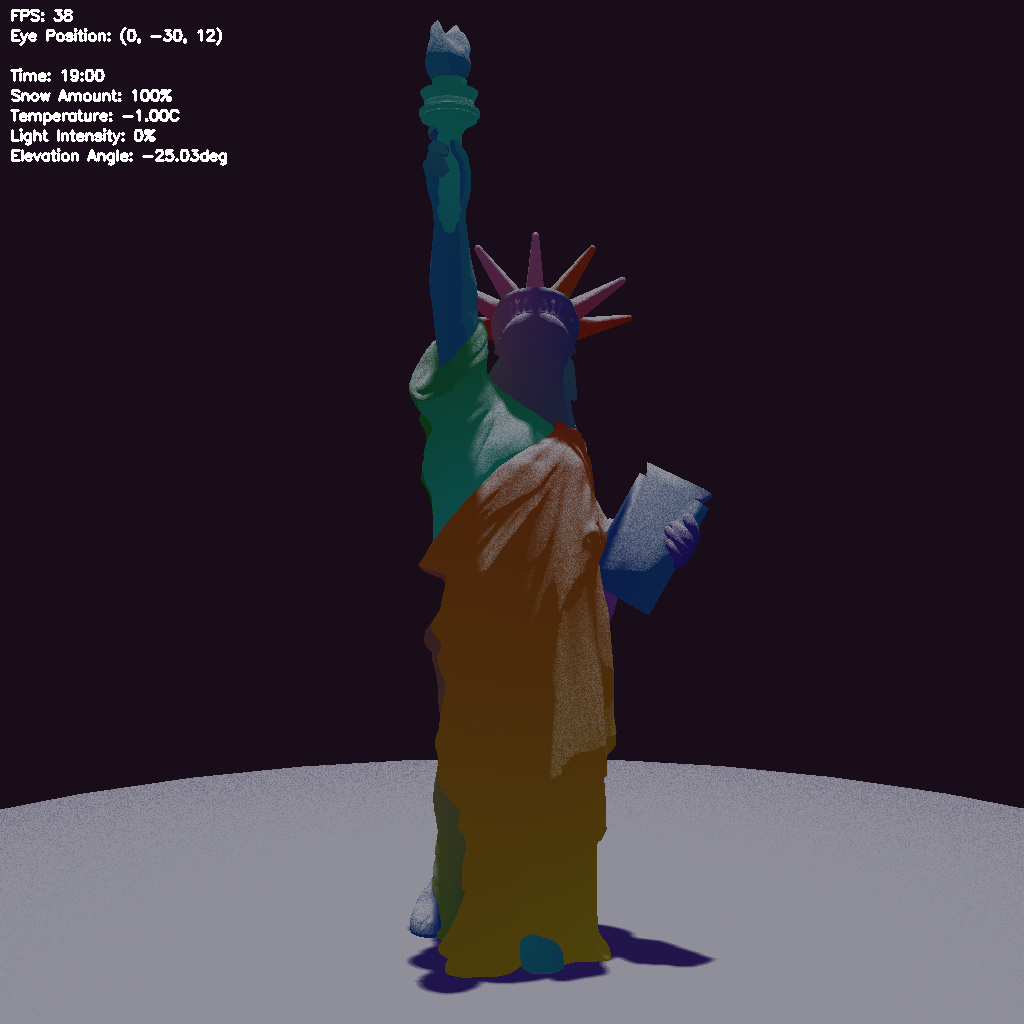
\includegraphics[width=0.33\textwidth]{images/T1900L35S.png}
    \label{fig:T1900L35S}
  }

  \caption{The rendered scene in different time (at 35 $^{\circ}$S on June \(22^{nd}\))}
  \label{fig:L35S}
\end{figure}
% Result 2: Snow Effect with Dynamic Daylight Simulation (Medium Latitude)

% Result 3: Snow Effect with Dynamic Daylight Simulation (High Latitude)
\subsection {Snow Effect with Dynamic Daylight Simulation (High Latitude)}

Figure 5 is the plot of the data at different times with a high latitude location on the summer solstice (60 $^{\circ}$N on June 
\(22^{nd}\)). The sunrise time is about 2:30 AM and the sunset time is about 9:30 PM, so there are 19 hours of daylight time.

\begin{figure}[h]
  \centering
  \begin{minipage}{1.00\textwidth}
      \centering
      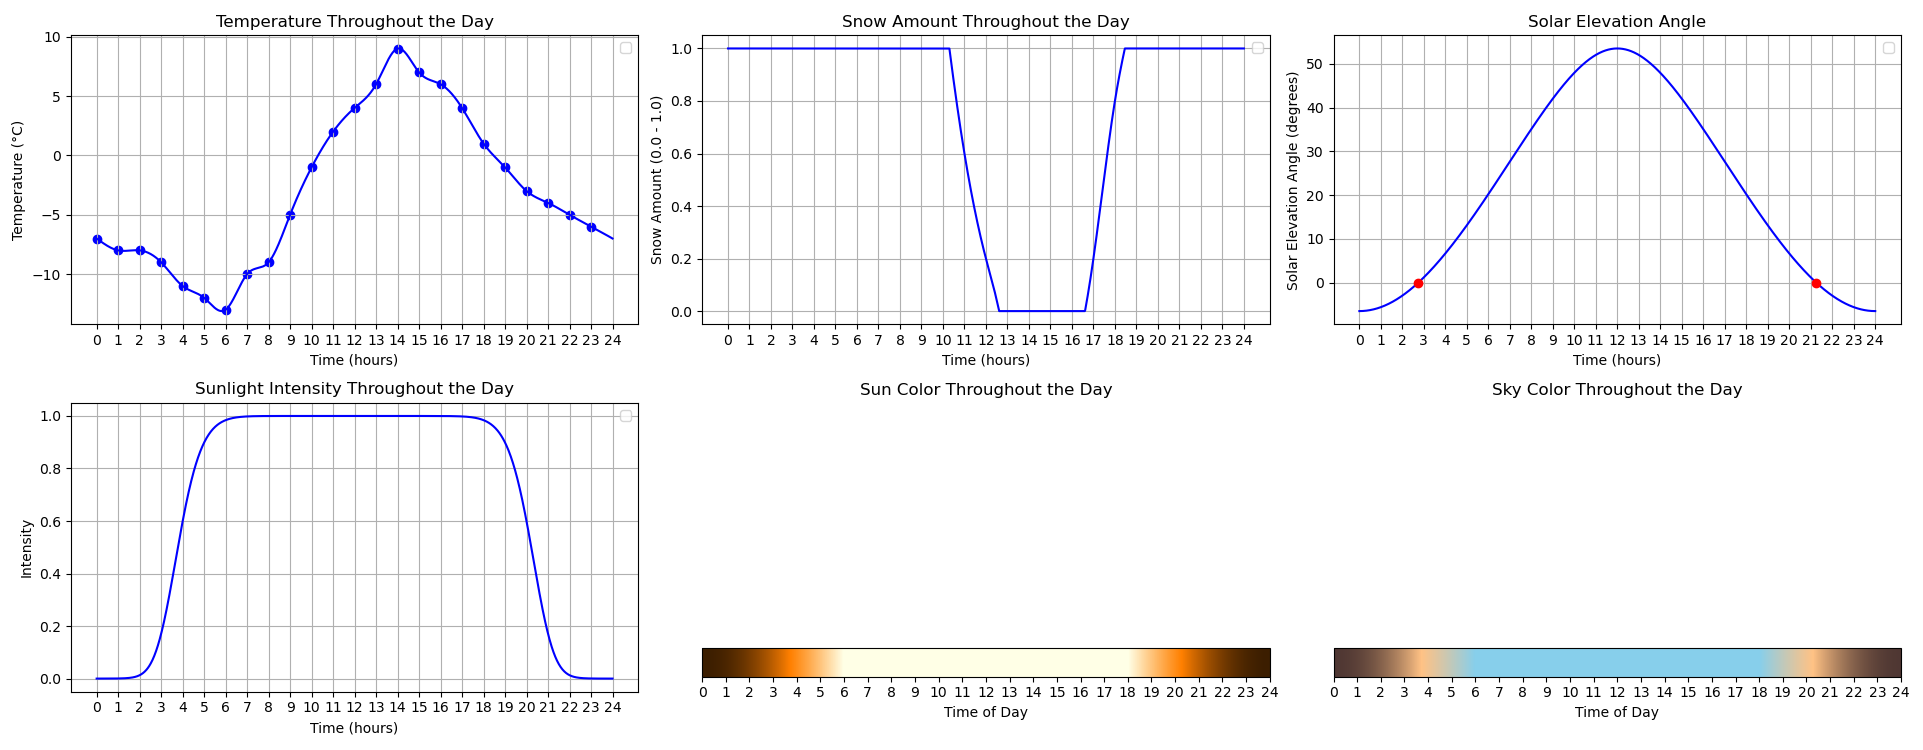
\includegraphics[width=\textwidth]{images/Plot60S.png}
      \caption{Relevant data in 60 $^{\circ}$N on June \(22^{nd}\)}
      \label{fig:Plot60S}
  \end{minipage}
\end{figure}

Figure 6 is the rendering effect. In the summer of the high-latitude locations, each day has a long daylight time. Throughout the 
night (e.g., midnight (a)), the sky is not completely dark even if the sun is below the horizon. At 8:00 AM (b), the sunlight 
intensity has already reached the maximum value. The scenes between the two locations are similar during the noon or afternoon time 
(c or d), except for the solar position. However, because of the high latitude, the sunlight intensity keeps the high value at 5:00 
PM (e) and finally starts dropping at around 7:00 PM (f).

\begin{figure}[h]
  \centering
  \subfloat[Time = 12:00 AM]{
    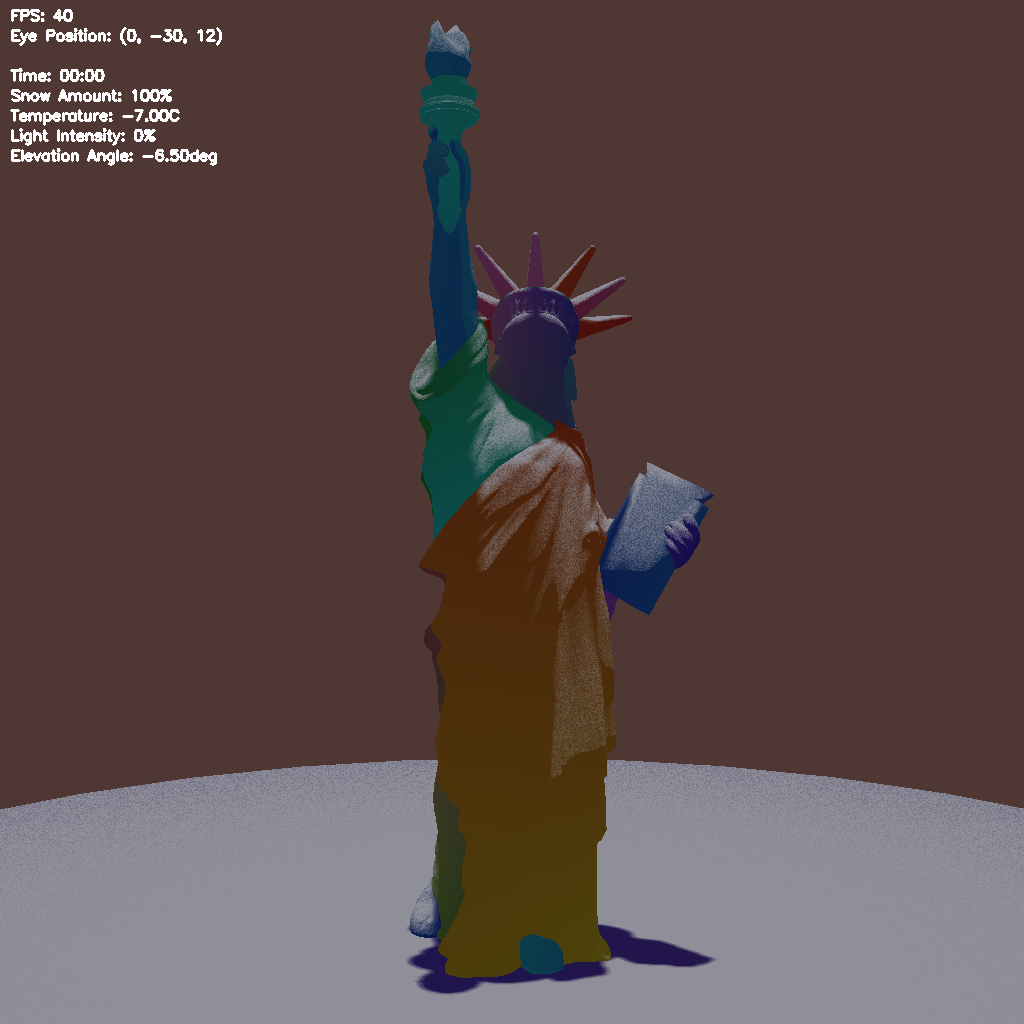
\includegraphics[width=0.3\textwidth]{images/T0000L60N.png}
    \label{fig:T0000L60N}
  }\hfill
  \subfloat[Time = 08:00 AM]{
    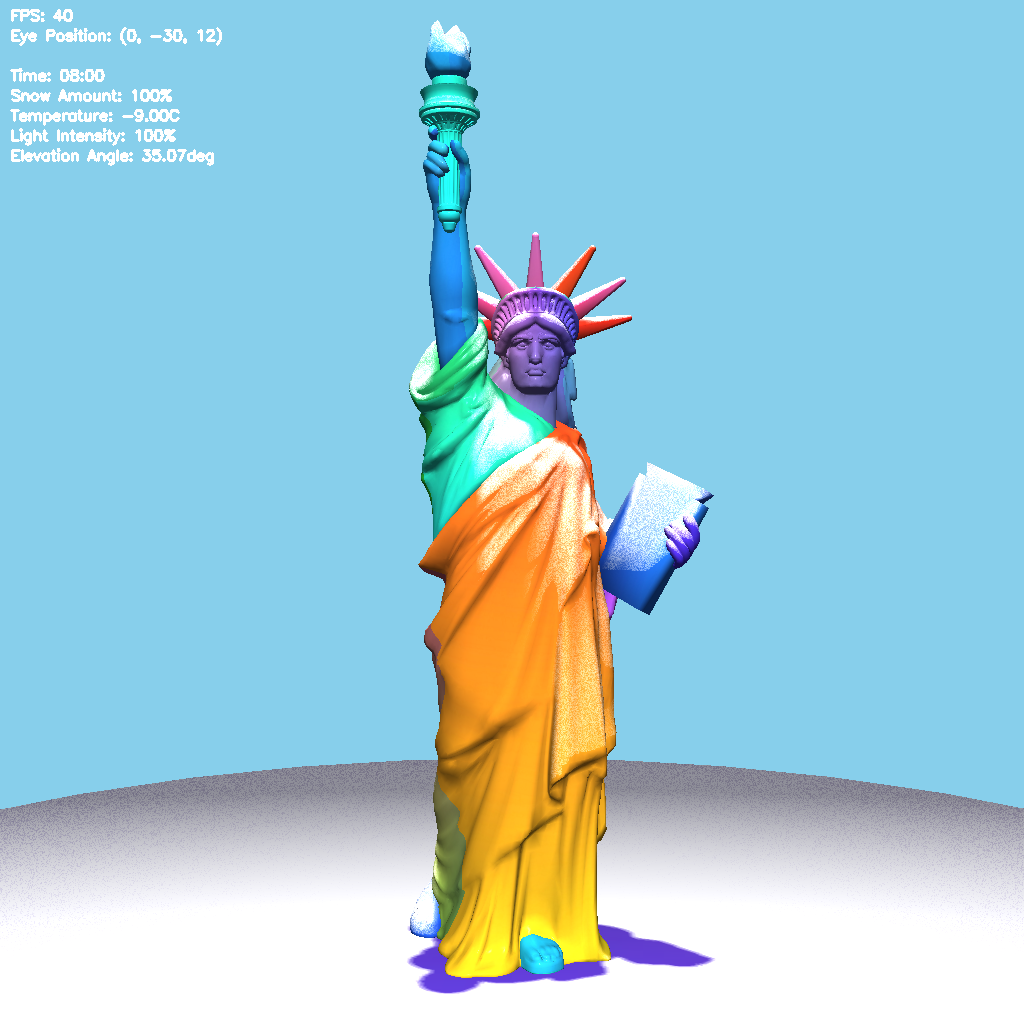
\includegraphics[width=0.3\textwidth]{images/T0800L60N.png}
    \label{fig:T0800L60N}
  }\hfill
  \subfloat[Time = 11:00 AM]{
    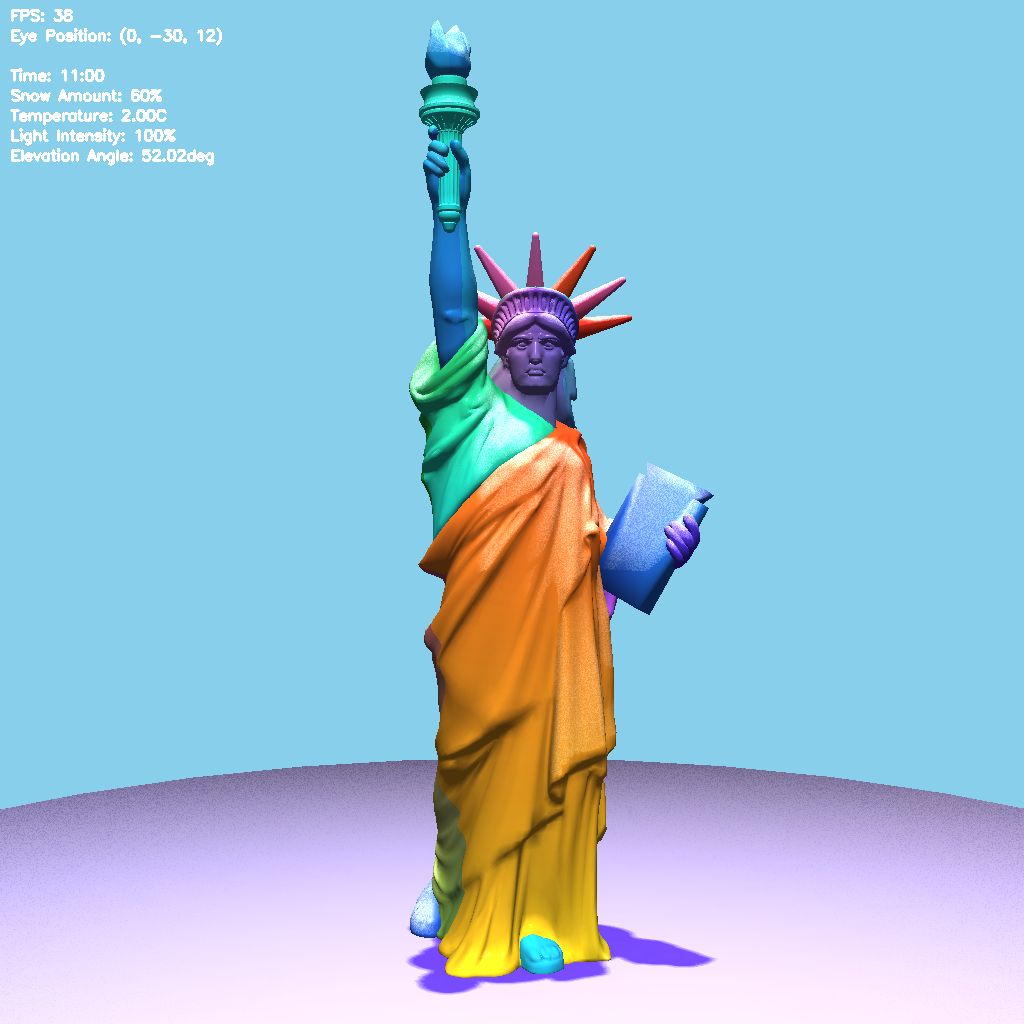
\includegraphics[width=0.3\textwidth]{images/T1100L60N.png}
    \label{fig:T1100L60N}
  }
  
  \subfloat[Time = 02:00 PM]{
    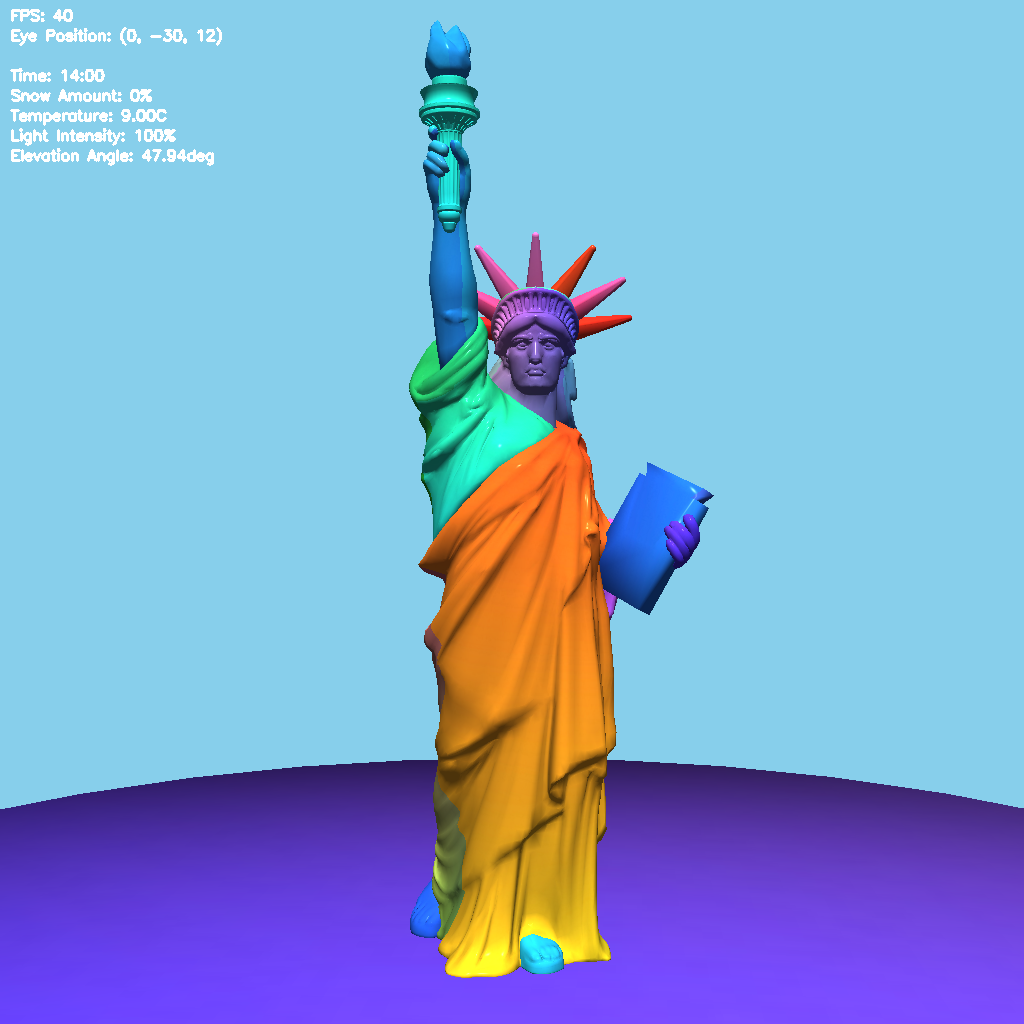
\includegraphics[width=0.3\textwidth]{images/T1400L60N.png}
    \label{fig:T1400L60N}
  }\hfill
  \subfloat[Time = 05:00 PM]{
    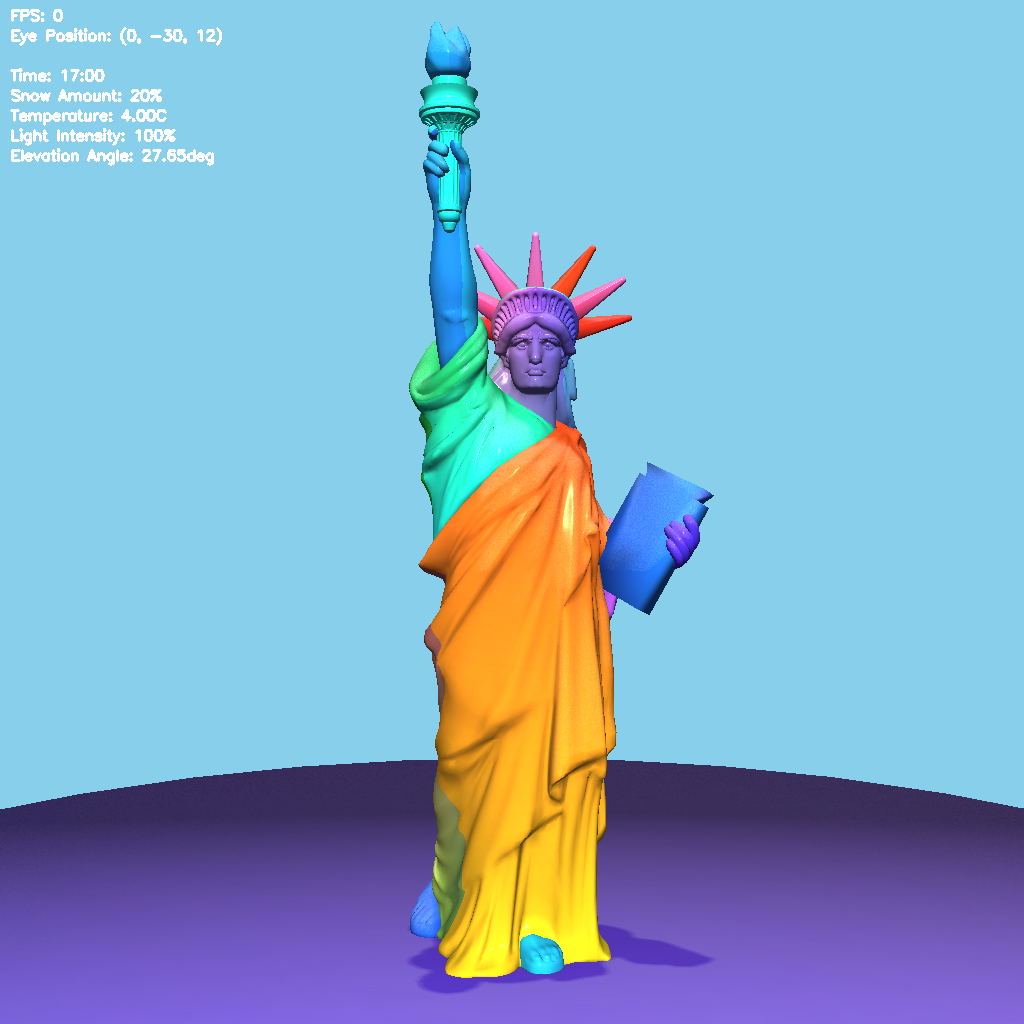
\includegraphics[width=0.3\textwidth]{images/T1700L60N.png}
    \label{fig:T1700L60N}
  }\hfill
  \subfloat[Time = 07:00 PM]{
    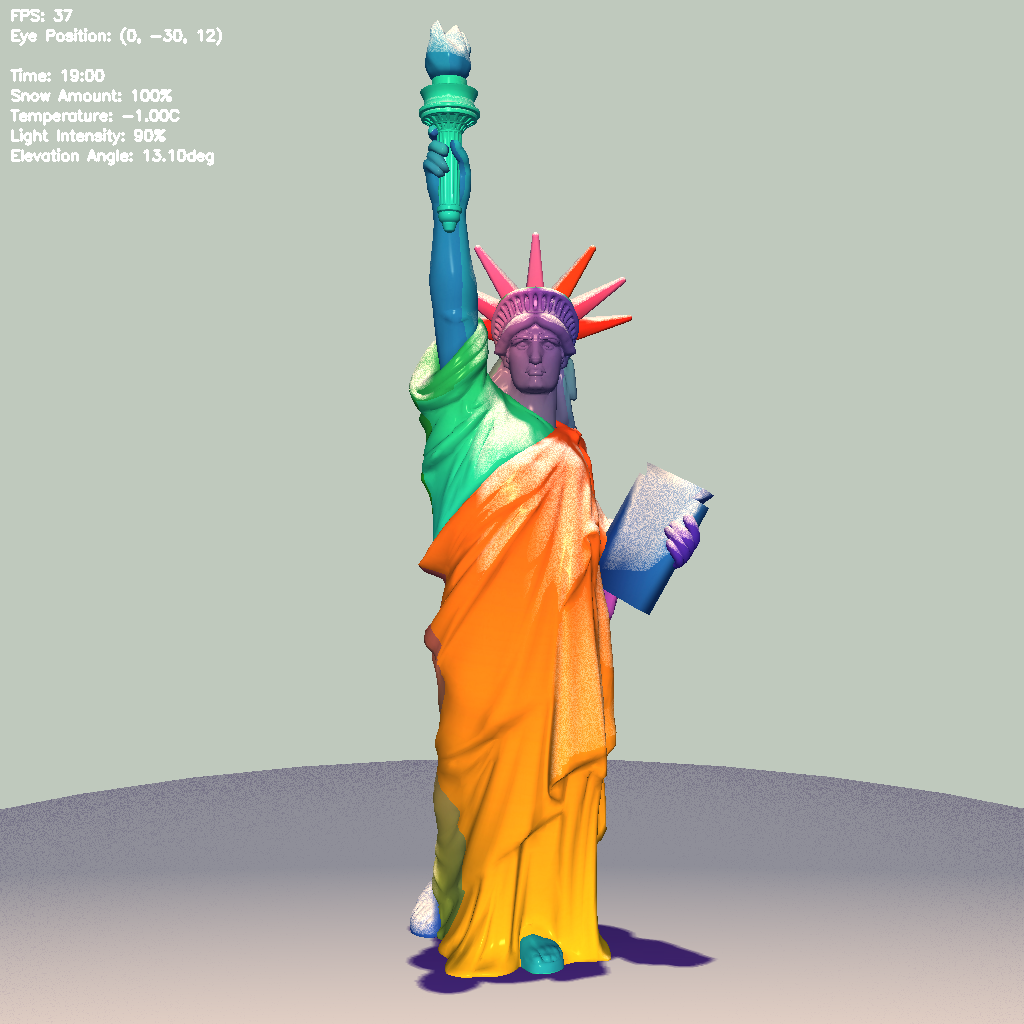
\includegraphics[width=0.3\textwidth]{images/T1900L60N.png}
    \label{fig:T1900L60N}
  }

  \caption{The rendered scene in different time (at 60 $^{\circ}$N on June \(22^{nd}\))}
  \label{fig:L60N}
\end{figure}
% Result 3: Snow Effect with Dynamic Daylight Simulation (High Latitude)

\section{Discussions}

% Discussion 1: Simulation Issues
\subsection {Simulation Issues}
In this paper, almost all the simulations are simplified for demonstrations only. For example, temperatures are only based on the data
of a single city and not bonded with the location parameters (e.g., altitude, latitude and ocean currents). Altitude and time zone
shift are not considered in the sunlight intensity formula, and snow is not simplify depends on temperature. To make a more precise
simulation, advanced knowledge of Physics, Mathematics, Geography, Astronomy and Meteorology is required and field measurements are
essential. New technologies like Machine Learning can also be used here.
% Discussion 1: Simulation Issues

% Discussion 2: Properties of the Snow TODO ref
\subsection {Properties of the Snow}
There are no special properties of the snow in this paper. However, for a better and more robust visual effect, they should be 
implemented. For example, a Snowy Realm should be full of thick snow. Feet and wheels should change the shape of the snow (e.g.,
footprints). If there is a war happening in the realm, the blood of wounded soldiers should dye snow red. When snow melts, water 
will be generated. Those special properties can be achieved by other techniques in Computer Graphics like texture mapping, vertex
displacement and ray tracing.
% Discussion 2: Properties of the Snow

% Discussion 3: Performance TODO ref
\subsection {Performance}
The code used in this paper achieves a satisfactory performance thanks to OpenGL, a modern open-source Computer Graphics Library, 
and improved computer hardware. The value of FPS reaches 40 when the window resolution is set to 900*900 (px) on an average laptop 
with an integrated GPU. This is much better than the paper. In that paper, the FPS value was only 1-3 with a window resolution of 
around 700*600 (px). However, this paper does not test complicated scenes like a Snowy Realm with a complex castle set.
% Discussion 3: Performance

\section{Conclusion}
This paper
\section{Future Work}

Fonts were the main cause of problems in the past years. Your PDF file must only
contain Type 1 or Embedded TrueType fonts. Here are a few instructions to
achieve this.


\section*{References}

{
\small

[1] Tan, Jian & Fan, Xiangtao. (2011). Particle System Based Snow Simulating in Real Time. Procedia Environmental Sciences. 
10. 1244–1249. 10.1016/j.proenv.2011.09.199. 


[2] Bower, J.M.\ \& Beeman, D.\ (1995) {\it The Book of GENESIS: Exploring
  Realistic Neural Models with the General Neural Simulation System.}  New York:
TELOS/Springer--Verlag.


[3] Hasselmo, M.E., Schnell, E.\ \& Barkai, E.\ (1995) Dynamics of learning and
recall at excitatory recurrent synapses and cholinergic modulation in rat
hippocampal region CA3. {\it Journal of Neuroscience} {\bf 15}(7):5249-5262.
}

\section*{Additional Experiment Results}

\section*{Confidential Peer Review} 

The percentage, who did what, ratio weights. 






\end{document}